% 中山大学科技类及IT类实验报告文档类(LaTeX模板)
\documentclass{sysucseexp}
\usepackage{fontspec,inconsolata,url}
\setmainfont{Times New Roman}
\setmonofont{Consolas}
% 载入需要的宏包
% =========引号宏包=========
\usepackage{csquotes}

% =========UML图宏包=========
\usepackage{pgf-umlcd}

% =========浮动体增强宏包=========
\usepackage{floatrow}
\usepackage{subcaption}% 子图排版

% =========命令行窗口及代码排版(自己开发的宏包)=========
\usepackage{boxie}

% =========插图标注宏包(修改为标注框可以换行)=========
\usepackage{tikz-imglabels}

% =========流程图宏包(自己开发)=========
\usepackage{tikz-flowchart}

%%% Local Variables:
%%% mode: latex
%%% TeX-master:"../main.tex"
%%% End:

% 进行必要的设置
% ====================================================================================
% cquotes宏包的中文引号样式
% ====================================================================================
\DeclareQuoteStyle{zhquotestyle}% style name
    {\symbol{"201C}}% opening outer mark
    {\symbol{"201D}}% closing outer mark
    {\symbol{"2018}}% opening inner mark
    {\symbol{"2019}}% closing inner mark

\setquotestyle{zhquotestyle}

% ====================================================================================
% 改变表格字体
% ====================================================================================
\BeforeBeginEnvironment{tabular}{\small}%

% ====================================================================================
% 设置floatrow浮动体属性
% ====================================================================================
\DeclareFloatVCode{beforefig}{\vspace{-4pt}}
\DeclareFloatVCode{beforetab}{\vspace{-6pt}}
\DeclareFloatVCode{afterfloat}{\vspace{4pt}}
\floatsetup{postcode=afterfloat}
\floatsetup[table]{capposition=TOP, captionskip=2pt, objectset=centering, margins=centering, precode=beforetab}
\floatsetup[figure]{captionskip=4pt, objectset=centering, margins=centering, precode=beforefig}

% ====================================================================================
% 代码交叉引用命令\autoref的引用格式
% ====================================================================================
\def\cvcounterautorefname{代码}%
\renewcommand{\thecvcounter}{\arabic{cvcounter}}
\def\cvcounterautorefname~#1\null{代码#1\null}%

%%% Local Variables:
%%% mode: latex
%%% TeX-master:"../main.tex"
%%% End:

% 专用术语宏命令进行必要的设置
% ====================================================================================
% 西北农林科技大学各单位名称
% ====================================================================================
\newcommand{\sysu}{中山大学}
\newcommand{\cse}{计算机学院}

% ============自定义专有名词命令============
\newcommand{\cl}{\texttt{C}语言}
\newcommand{\ccpp}{\texttt{C/C++}}
\newcommand{\win}{\texttt{Windows}}
\newcommand{\ide}{\texttt{IDE}}
\newcommand{\gcc}{\texttt{GCC}}
\newcommand{\gpp}{\texttt{G++}}
\newcommand{\gnu}{\texttt{GNU}}
\newcommand{\cb}{\texttt{Code::Blocks}}
\newcommand{\mgww}{\texttt{MinGW}}
\newcommand{\mgw}{\texttt{MinGW32}}
\newcommand{\mgwww}{\texttt{MinGW-w64}}
\newcommand{\lumos}{\texttt{Linux}、\texttt{Unix}、\texttt{Mac OS}}
\newcommand{\unix}{\texttt{UNIX}}
\newcommand{\lnx}{\texttt{Linux}}
\newcommand{\mk}{\texttt{make}}
\newcommand{\ph}{\texttt{Path}}
\newcommand{\cmdd}{\texttt{cmd}}
\newcommand{\gdb}{\texttt{gdb}调试器}
\newcommand{\vside}{\texttt{Visual Studio}}
\newcommand{\mfile}{\texttt{Makefile}}
\newcommand{\tgt}{\texttt{target}}
\newcommand{\prqt}{\texttt{prerequisites}}
\newcommand{\cbv}{\texttt{17.12}}
\newcommand{\db}{\texttt{DEBUG}}
\newcommand{\dbger}{\texttt{Debugger}}
\newcommand{\cdb}{\texttt{cdb}调试器}
\newcommand{\gdbcmd}{\texttt{(gdb)}}
\newcommand{\bug}{\texttt{BUG}}
\newcommand{\ieee}{\texttt{IEEE754}标准}
\newcommand{\ascii}{\texttt{ASCII}}
\newcommand\vararg{变长形参列表}
\newcommand\varargfun{\vararg{}函数}
\newcommand{\cg}{\texttt{CGraph2D} 图形库}
\newcommand{\git}{分布式版本控制系统\texttt{Git}}
\newcommand{\github}{\texttt{Github}平台}
% ====================================


%%% Local Variables:
%%% mode: latex
%%% TeX-master:"../main.tex"
%%% End:


% 设置封面基本信息,\linebreak 前面不要有空格,
% 中文之间的空格无法消除
% 另,在\sysucseset中不可以出现空行
\sysucseset{
  college = {计算机学院},            % 学院名称
  projname = {操作系统原理实验},       % 实践课程名称
  title = {进程调度算法},    % 实验报告题目
  stuno = {21307443},              % 学号
  author = {叶文洁},             % 姓名
  major = {计算机科学与技术},          % 专业
  adviser = {刘慈欣},                   % 指导教师姓名
  startdate = {2023年3月1日},        % 实验起始日期
  enddate = {4月1日},        % 实验结束日期
  labroom = {实验中心D503}
}

\begin{document} %在document环境中撰写文档

%%%%%%%%%%%%%%%%%%%%%%%%%%%%%%%%%%%%%%%%
% 封面及目录,无需改动此处代码
% 面页,需要在导言区用\sysucseset命令填写基本信息
\makecover
% 目录
\tableofcontents
\cleardoublepage
% 设置正文页眉页脚格式,并重新设置页码为1
\pagestyle{main} % 无页眉,页码在页脚居中
%%%%%%%%%%%%%%%%%%%%%%%%%%%%%%%%%%%%%%%%

% 排版正文内容
\section{实验概述}
在本次实验中,同学们会熟悉现有Linux内核的编译过程和启动过程, 并在自行编译内核的基础上构建简单应用并启动。
同时,同学们会利用精简的Busybox工具集构建简单的OS, 熟悉现代操作系统的构建过程。 此外,同学们会熟悉编译环境、相关工具集,并能够实现内核远程调试。
\section{实验任务}
\begin{enumerate}
  \item 搭建OS内核开发环境包括:代码编辑环境、编译环境、运行环境、调试环境等。
  \item 下载并编译i386(32位)内核,并利用qemu启动内核。
  \item 熟悉制作initramfs的方法。
  \item 编写简单应用程序随内核启动运行。
  \item 编译i386版本的Busybox,随内核启动,构建简单的OS。
  \item 开启远程调试功能,进行调试跟踪代码运行。
  \end{enumerate}

\section{模板使用样例}
\subsection{插图排版}
在\enquote{sysucseexp.cls}模板中,除了可以使用普通的figure浮动体环境
结合graphicx宏包实现插图排版外,还可以使用floatrow增强浮动体宏包进行浮
动体排版(适合多图并排、子图排版等)。有关该宏包的使用细节,请在命令行使
用\enquote{texdoc floatrow}命令查看其使用说明书。例如,可以
用\autoref{texcode01}排版\autoref{sharefig:a}。

% 该center环境中的代码为排版示例代码,实际排版中不需要该代码
\begin{center}
\begin{langCVOne}[tex][texcode01][\LaTeX{}]{排版单一插图浮动体}
  \begin{figure}[!htp]
    \begin{floatrow}
      \ffigbox[\FBwidth]{
        \includegraphics[width=0.4\textwidth]{example-image-a}
      }{\caption{一个插图}\label{sharefig:a}}
    \end{floatrow}
  \end{figure}
\end{langCVOne}
\end{center}

\begin{figure}[!htp]
  \begin{floatrow}
    \ffigbox[\FBwidth]{
      \includegraphics[width=0.4\textwidth]{example-image-a}
    }{\caption{一个插图}\label{sharefig:a}}
  \end{floatrow}
\end{figure}

当然,也可以用\autoref{texcode02}排版带有子图的\autoref{trifig}。  

% 该center环境中的代码为排版示例代码,实际排版中不需要该代码
\begin{center}
\begin{langCVOne}[tex][texcode02][\LaTeX{}]{排版单一插图浮动体}
\begin{figure}[!htp]
  \ffigbox[\textwidth]%
  {%
    \begin{subfloatrow}[2]%\useFCwidth
      \ffigbox[\FBwidth]{
        \includegraphics[width=0.3\textwidth]{example-image-a}
      }{\caption{子题注1}\label{trifig:a}}
      \ffigbox[\FBwidth]{
        \includegraphics[width=0.3\textwidth]{example-image-b}
      }{\caption{子题注2}\label{trifig:b}}
    \end{subfloatrow}    
    \begin{subfloatrow}[2]%\useFCwidth      
      \ffigbox[\FBwidth]{
        \includegraphics[width=0.3\textwidth]{example-image-c}
      }{\caption{子题注3}\label{trifig:c}}
      \ffigbox[\FBwidth]{
        \includegraphics[width=0.3\textwidth]{example-image}
      }{\caption{子题注4}\label{trifig:d}}
    \end{subfloatrow}
  }{\caption{四个子图}\label{trifig}}
\end{figure}
\end{langCVOne}
\end{center}

\begin{figure}[!htp]
  \ffigbox[\textwidth]%
  {%
    \begin{subfloatrow}[2]%\useFCwidth
      \ffigbox[\FBwidth]{
        \includegraphics[width=0.25\textwidth]{example-image-a}
      }{\caption{子题注1}\label{trifig:a}}
      \ffigbox[\FBwidth]{
        \includegraphics[width=0.25\textwidth]{example-image-b}
        
      }{\caption{子题注2}\label{trifig:b}}
    \end{subfloatrow}    
    \begin{subfloatrow}[2]%\useFCwidth      
      \ffigbox[\FBwidth]{
        \includegraphics[width=0.25\textwidth]{example-image-c}
      }{\caption{子题注3}\label{trifig:c}}
      \ffigbox[\FBwidth]{
        \includegraphics[width=0.25\textwidth]{example-image}
      }{\caption{子题注4}\label{trifig:d}}
    \end{subfloatrow}
  }{\caption{四个子图}\label{trifig}}
\end{figure}

在模板中,已为插图设置
了{{./figs/}、{./figure/}、{./figures/}、{./image/}、{./images/}、
  {./graphics/}、{./graphic/}、{./pictures/}、{./picture/}}相对路径,可
以在当前工作路径中任意一个这样命名的文件夹,以存放需要的插图文件。
如果需要插入一个简单的表格,可以仅使用{table}和{tabular}环境实现,如%
\autoref{tab:city}。

\subsection{表格排版}
\emph{注意:}科技文档中的表格需要采用\emph{三线表}。
\begin{table}[!htb]
  \caption[城市人口]{城市人口数量排名 (source: Wikipedia)\label{tab:city}}
  \begin{tabular}{lr}
    \toprule
    城市 & 人口 \\
    \midrule
    Mexico City & 20,116,842\\
    Shanghai & 19,210,000\\
    Peking & 15,796,450\\
    Istanbul & 14,160,467\\
    \bottomrule
  \end{tabular}
\end{table}

如果多个表格布局较为复杂,可以使用floatrow宏包实现排版。如%
用\autoref{texcodetab}可编制\autoref{tab:testsample}和%
\autoref{tab:city2}所示的横向并排表格。%

% 该center环境中的代码为排版示例代码,实际排版中不需要该代码
\begin{center}
  \begin{langCVOne}[tex][texcodetab][\LaTeX{}]{表格排版}
    % 横向排版两个表格
    \begin{table}[!htp]
      \begin{floatrow}
        \ttabbox[\FBwidth]
        {
          \begin{tabular}{ccl}
            \toprule
            序号 & 测试用例 & \multicolumn{1}{c}{测试目的}\\
            \midrule
            1 & a & 小写字母到大写字母转换\\
            2 & A & 大写字母到小写字母转换\\
            3 & @ & 非字母字符测试\\
            4 & 2 & 非字母其它字符\\
            \bottomrule
          \end{tabular}      
        }{\caption{字母大小写转换测试用例表}\label{tab:testsample}}
        \ttabbox[\FBwidth]
        {
          \begin{tabular}{lr}
            \toprule
            城市 & 人口 \\
            \midrule
            Mexico City & 20,116,842\\
            Shanghai & 19,210,000\\
            Peking & 15,796,450\\
            Istanbul & 14,160,467\\
            \bottomrule
          \end{tabular}      
        }{\caption{城市人口数量排名}\label{tab:city2}}
      \end{floatrow}
    \end{table}
  \end{langCVOne}
\end{center}

% 横向排版两个表格
\begin{table}[!htp]
  \begin{floatrow}
    \ttabbox[\FBwidth]
    {
      \begin{tabular}{ccl}
        \toprule
        序号 & 测试用例 & \multicolumn{1}{c}{测试目的}\\
        \midrule
        1 & a & 小写字母到大写字母转换\\
        2 & A & 大写字母到小写字母转换\\
        3 & @ & 非字母字符测试\\
        4 & 2 & 非字母其它字符\\
        \bottomrule
      \end{tabular}      
    }{\caption{字母大小写转换测试用例表}\label{tab:testsample}}
    \ttabbox[\FBwidth]
    {
      \begin{tabular}{lr}
        \toprule
        城市 & 人口 \\
        \midrule
        Mexico City & 20,116,842\\
        Shanghai & 19,210,000\\
        Peking & 15,796,450\\
        Istanbul & 14,160,467\\
        \bottomrule
      \end{tabular}      
    }{\caption{城市人口数量排名}\label{tab:city2}}
  \end{floatrow}
\end{table}
如果表格内容很多,导致无法放在一页内的话,需要用{longtable} 或{longtabu} 进行分页。
\subsection{项目符号和步骤分点排版}
在\enquote{sysucseexp.cls}模板中,基于enumitem宏包分别对itemize、
enumerate和description三个环境的各个距离参数进行了修正,以使其排版结果
符合中文习惯的首行缩进格式。
\subsubsection{itemize环境}
\begin{itemize}
\item 床前明月光。
\item 疑是地上霜。
\item 举头望明月。
\item 低头思故乡。
\end{itemize}
\subsubsection{enumerate环境}
\begin{enumerate}
\item 床前明月光。
\item 疑是地上霜。
\item 举头望明月。
\item 低头思故乡。
\end{enumerate}
\subsubsection{description环境}
\begin{description}
\item[床前明月光] 我欲乘风归去。
\item[疑是地上霜] 又恐琼楼玉宇。
\item[举头望明月] 高处不胜寒。
\item[低头思故乡] 起舞弄清影。
\end{description}
\subsection{文本框排版}
文本框盒子继承于自己开发的boxie宏包,可用于实验心得总结或注意事项说明。
其使用细节请在\github{}查看\href{https://github.com/registor/boxiesty}{boxie宏包}的使用说明书。
同时,在该宏包的基础上,为boxie宏包添加加了摘自于
\href{https://github.com/WisdomFusion/latex-templates/tree/master/progartcn}{progartcn
  论文模板}的\enquote{标题}、\enquote{注意}、\enquote{重要}、
\enquote{技巧}和\enquote{警告}文本框环境代码\footnote{本节示例摘自于
  该模板中的tutorial-sample.tex文件}。
\subsubsection{\enquote{标题}文本框}
标题文本框环境的使用格式为:

\verb|\begin{titledBox}{<title>} <content> \end{titledBox}|

\begin{titledBox}{HTTP/Console 内核}
  HTTP 内核继承自 \verb|Illuminate\Foundation\Http\Kernel| 类,该类定义了一个 \verb|bootstrappers| 数组,这个数组中的类在请求被执行前运行,这些 \verb|bootstrappers| 配置了错误处理、日志、检测应用环境以及其它在请求被处理前需要执行的任务。
\end{titledBox}
\subsubsection{\enquote{注意}文本框}
注意文本框环境的使用格式为:

\verb|\begin{noteBox} <content> \end{noteBox}|

\begin{noteBox}
  HTTP 内核继承自 \verb|Illuminate\Foundation\Http\Kernel| 类,该类定义了一个 \verb|bootstrappers| 数组,这个数组中的类在请求被执行前运行,这些 \verb|bootstrappers| 配置了错误处理、日志、检测应用环境以及其它在请求被处理前需要执行的任务。
\end{noteBox}

\subsubsection{\enquote{重要}文本框}
重要文本框环境的使用格式为:

\verb|\begin{importantBox} <content> \end{importantBox}|

\begin{importantBox}
  HTTP 内核继承自 \verb|Illuminate\Foundation\Http\Kernel| 类,该类定义了一个 \verb|bootstrappers| 数组,这个数组中的类在请求被执行前运行,这些 \verb|bootstrappers| 配置了错误处理、日志、检测应用环境以及其它在请求被处理前需要执行的任务。
\end{importantBox}
\subsubsection{\enquote{技巧}文本框}
技巧文本框环境的使用格式为:

\verb|\begin{tipBox} <content> \end{tipBox}|

\begin{tipBox}
  HTTP 内核继承自 \verb|Illuminate\Foundation\Http\Kernel| 类,该类定义了一个 \verb|bootstrappers| 数组,这个数组中的类在请求被执行前运行,这些 \verb|bootstrappers| 配置了错误处理、日志、检测应用环境以及其它在请求被处理前需要执行的任务。
\end{tipBox}
\subsubsection{\enquote{警告}文本框}
警告文本框环境的使用格式为:

\verb|\begin{warningBox} <content> \end{warningBox}|

\begin{warningBox}
  HTTP 内核继承自 \verb|Illuminate\Foundation\Http\Kernel| 类,该类定义了一个 \verb|bootstrappers| 数组,这个数组中的类在请求被执行前运行,这些 \verb|bootstrappers| 配置了错误处理、日志、检测应用环境以及其它在请求被处理前需要执行的任务。
\end{warningBox}

\subsection{补充:模板文件夹中的重要文件}
\begin{importantBox}
  在使用在\enquote{sysucseexp.cls}模板前请确保:
  \verb|sysucseexp.cls|模板文件在当前工作文件夹中。
  
  如果需要代码盒子等各类盒子排版,则需要确保\verb|boxie.sty|、
  \verb|fvextra.sty|、\verb|lstlinebgrd.sty|
  这3个宏包文件在当前工作文件夹中,并且需要引入\verb|boxie|宏包,
  \verb|boxie|宏包会根据需要加载\verb|fvextra|和\verb|lstlinebgrd|
  宏包,这两个宏包无需手动加载。
  
  如果需要绘制UML图,则需要加载\verb|pgf-umlcd|宏包,此时需要确保\verb|pgf-umlcd.sty|
  宏包文件在当前工作文件夹中(TeXLive自带的宏包无法正确处理中文类名称,同时,
  修改了其association命令,以符合龚晓庆教材绘图习惯)。
  
  如果需要绘制流程图,则需要加载\verb|tikz-flowchart|宏包,此时需要确保\verb|tikz-flowchart.sty|
  宏包文件在当前工作文件夹中。
  
  如果需要为插图进行标注,则需要加载\verb|tikz-imglabels|宏包,此时需要确保\verb|tikz-imglabels.sty|
  宏包文件在当前工作文件夹中(TeXLive自带的宏包无法正确标注中的换行问题)。

  \verb|Makefile|文件是执行make命令需要的脚本文件,可以根据需要选择。

  \verb|.latexmkrc|文件是执行latexmk命令需要的脚本文件,可以根据需要选择。
\end{importantBox}

\subsection{代码排版}
\begin{importantBox}
  由于需要排版代码文件,建议使用minted宏包实现代码排版,因此请确保安装
  有Python及其Pygments模块,详情请使用\verb|texdoc minted|命令查看
  minted宏包的使用说明。
  同时,为支持minted编译,请使用\verb|-shell-escape|编译参数。  
\end{importantBox}
可以使用boxie宏包提供的langPyOne、langCVOne等环境或langPyfile和langCVfile等命令实现嵌入式代码或来自文件代码的排版。Py系列环境和命令不带引用计数
和标签,CV系列环境和命令带有引用计数和标签。如果需要交叉引用和参考文献,建议按如下方式执行4次编译:
\subsubsection{使用minted宏包排版代码}
\begin{ubtdark}{4次编译}
  xelatex -shell-escape main.tex
  biber main
  xelatex -shell-escape main.tex
  xelatex -shell-escape main.tex
\end{ubtdark}

\subsubsection{使用listings宏包排版代码}
\begin{ubtdark}{4次编译}
  xelatex main.tex
  biber main
  xelatex main.tex
  xelatex main.tex
\end{ubtdark}

\subsubsection{插入行间的命令行代码}
命令行代码的插入方式为:
\verb|\begin{ubtdark} <content> \end{ubtdark}|
下面提供两个例子:如果需要运行C++测试程序,则执行如下命令:
\begin{ubtdark}{运行命令}
  make run
\end{ubtdark}

如果使用\verb|.latexmkrc|,则执行latexmk命令即可:
\begin{ubtdark}{编译latex}
  latexmk
\end{ubtdark}

\subsubsection{以嵌入源码的方式插入代码}
例如,使用langPyOne环境可以排版不带引用计数和标签的代码。在方框内可指定语言,如果是插入C/C++语言,则参数为C++;如果是插入x86汇编语言,
则参数为[x86masm]Assembler。例如下面,插入了一段C++代码:
\begin{langPyOne}[C++]{基于范围的循环}
int main(){
    // 累加 20 以内的素数
    int sum = 0;
    for(int e : {2, 3, 5, 7, 11, 13, 17, 19}){ 
        sum += e;
    }
    cout << sum << endl;
    int arr[] = {1, 3, 5, 7, 9};
    // 声明数组 arr,初始化为 5 个奇数
    for(auto &ele : arr){
        // 声明 ele,与数组 arr 关联在一起,用了 auto
        ele = ele * 2;
        // 修改数组每个元素的值
        cout << ele << " ";
        // 输出 ele,2 6 10 14 18
    }
    cout << endl;
    for(auto ele : arr){
        cout << ele << " ";
    }
    // 没有改变:1 3 5 7 9
    cout << endl;
    return 0;
}  
\end{langPyOne}

再如,使用langCVOne环境可以排版带有引用计数和标签的代码,如\autoref{code:ex04-01}。
\begin{langCVOne}[[x86masm]Assembler][code:ex04-01][asm]{汇编测试程序}
cin:
  mov ah,0x00  ;从键盘读入字符
  int 16h
  cmp al,0x1b  ;0x1b表示的是esc按键
  je end
  mov ah,0x02  ;移动光标
  int 10h
  mov ah,0x09  ;在当前位置写字符
  int 10h
  add dl,1
  cmp dl,0x50  ;已经超80列
  je newl
  jmp cin
newl: 
  add dh,1     ;换行
  mov dl,0x00
  cmp dh,0x19  ;已经超25行
  je end
  jmp cin
end:
\end{langCVOne}

\subsubsection{以源码文件URI的方式插入代码}
代码排版命令用于根据代码文件进行排版,因此,可以在IDE中,例如
Code::Blocks中对代码进行排版,然后将排版后的文件直接用代码排版命令在
\LaTeX{}中进行排版。
例如,使用langPyfile命令可以载入代码文件,排版不带引用计数和标签的代码
(注意指定必要的路径)。

\langPyfile{基于范围的循环}{codes/ex04-01.cpp}

再如,使用langCVfile命令可以载入代码文件,排版带引用计数和标签的代码
(注意指定必要的路径),如\autoref{code:ex04-02}。

\langCVfile[[x86masm]Assembler][code:ex04-02][asm]{MBR加载程序}{codes/mbr.asm}

注:使用minted宏包排版C++代码,可以使用c++/C++或cpp指定语言名称,若使
用listings宏包排版代码,则只能使用c++/C++指定语言名称。如果使用TeXstudio、VSCode等IDE工具,请参阅相关资料对IDE进行必要的配置。

\section{实验步骤与实验结果}
\subsection{实验任务1——复现bootloader加载过程}
\begin{titledBox}{任务要求}
  复现"加载bootloader"一节,说说你是怎么做的并提供结果截图,也可以参考Ucore、Xv6等系统源码,实现自己的LBA方式的磁盘访问。
\end{titledBox}
\subsubsection{步骤一}
首先,我们需要安装C++编译工具,安装命令如下:
\begin{ubtdark}{安装编译工具}
  sudo apt install libssl-dev
  sudo apt install libc6-dev-i386
  sudo apt install gcc-multilib 
  sudo apt install g++-multilib
\end{ubtdark}
\subsubsection{步骤二}
然后,我们需要将内核编译成i386 32位版本。执行命令行如下:
\begin{ubtdark}{将内核编译成i386 32位版本}
  make i386_defconfig
  make menuconfig
\end{ubtdark}
\subsection{实验任务2——采用CHS方式读取硬盘}
\begin{titledBox}{任务要求}
  在"加载bootloader"一节中,我们使用了LBA28的方式来读取硬盘。此时,我们只要给出逻辑扇区号即可,但需要手动去读取I/O端口。然而,BIOS提供了实模式下读取硬盘的中断,其不需要关心具体的I/O端口,只需要给出逻辑扇区号对应的磁头(Heads)、扇区(Sectors)和柱面(Cylinder)即可,又被称为CHS模式。现在,同学们需要将LBA28读取硬盘的方式换成CHS读取,同时给出逻辑扇区号向CHS的转换公式。最后说说你是怎么做的并提供结果截图。
\end{titledBox}
\subsubsection{步骤一}
首先,我们需要安装C++编译工具,安装命令如下:
\begin{ubtdark}{安装编译工具}
  sudo apt install libssl-dev
  sudo apt install libc6-dev-i386
  sudo apt install gcc-multilib 
  sudo apt install g++-multilib
\end{ubtdark}
\subsubsection{步骤二}
然后,我们需要将内核编译成i386 32位版本。执行命令行如下:
\begin{ubtdark}{将内核编译成i386 32位版本}
  make i386_defconfig
  make menuconfig
\end{ubtdark}

\subsection{实验任务3——进入保护模式}
\begin{titledBox}{任务要求}
  复现“进入保护模式”一节,使用gdb或其他debug工具在进入保护模式的4个重要步骤上设置断点,并结合代码、寄存器的内容等来分析这4个步骤,最后附上结果截图。gdb的使用可以参考指导网站appendix中的“debug with gdb and qemu”。
\end{titledBox}

\subsubsection{步骤一}
首先,我们需要安装C++编译工具,安装命令如下:
\begin{ubtdark}{安装编译工具}
  sudo apt install libssl-dev
  sudo apt install libc6-dev-i386
  sudo apt install gcc-multilib 
  sudo apt install g++-multilib
\end{ubtdark}
\subsubsection{步骤二}
然后,我们需要将内核编译成i386 32位版本。执行命令行如下:
\begin{ubtdark}{将内核编译成i386 32位版本}
  make i386_defconfig
  make menuconfig
\end{ubtdark}

\subsection{实验任务4——保护模式下的汇编程序设计}
在进入保护模式后,按照如下要求,编写并执行一个自己定义的32位汇编程序,要求简单说一说你的实现思路,并提供结果截图。
\begin{titledBox}{任务要求}
  使用两种不同的自定义颜色和一个自定义的起始位置$(x,y)$,使得bootloader加载后,在显示屏坐标$(x,y)$处开始输出自己的学号+姓名拼音首字母缩写,要求相邻字符前景色和背景色必须是相互对调的。
\end{titledBox}
\subsubsection{步骤一}
首先是汇编程序的设计思路:
\begin{enumerate}
  \item 首先,考虑到32位地址下,。。。
  \item 然后,。。。
  \item 最后,。。。。
\end{enumerate}
结合上述设计思路,编码得到的汇编程序段如下:
\begin{center}
  \begin{langCVOne}[[x86masm]Assembler][asmcode01][asm]{实验任务4汇编}
    my_function:
    push ax
    push bx
    
    sub ax, 10
    sub bx, 10
    ; 后进先出
    pop ax
    ret
  \end{langCVOne}
  \end{center}
\subsubsection{步骤二}
接着,通过执行下面的命令编译并运行汇编程序:
\begin{ubtdark}{编译并利用QEMU运行程序}
  nasm -o mbr.o -g -f elf32 mbr.asm 
  ld -o mbr.symbol -melf_i386 -N mbr.o -Ttext 0x7c00
  qemu-system-i386 -hda hd.img -s -S -parallel stdio -serial null
\end{ubtdark}

执行汇编程序后,可得到\autoref{fig:result}所示的结果:
\begin{figure}[H]
  \begin{floatrow}
    \ffigbox[\FBwidth]{
      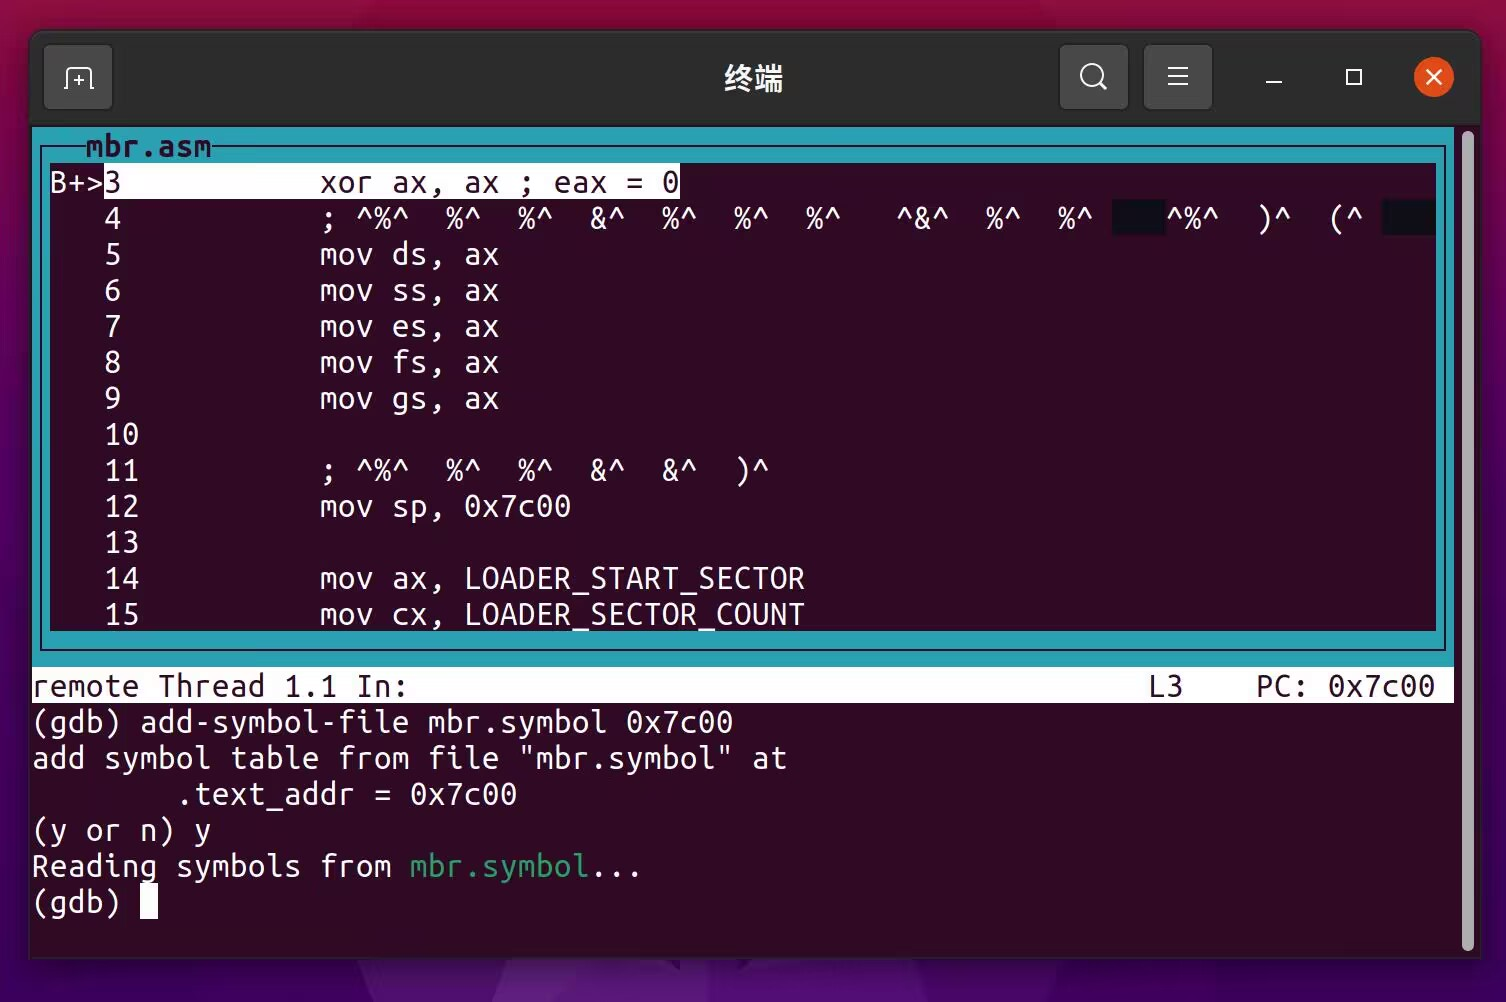
\includegraphics[width=0.6\textwidth]{figs/result.jpg}
    }{\caption{实验结果}
    \label{fig:result}}
  \end{floatrow}
\end{figure}

\section{实验总结与心得}
通过本次实验,我解决了中大学子在撰写实验报告时的排版问题,减轻了排版工作量,排版结果更标准、更专业......

\section{附录:实验代码清单}\label{secboxiety}
实验任务1的C++代码如下:
\langCVfile[C++][code:ex0402][C++]{实验任务1}{codes/ex04-01.cpp}
实验任务2的汇编代码如下:
\langCVfile[[x86masm]Assembler][code:ex0404][asm]{实验任务2}{codes/mbr.asm}

\section{参考文献及资料}
\begin{itemize}
  \item x86汇编语言——从实模式到保护模式. 李忠等. 电子工业出版社
  \item 第三章-从实模式到保护模式 
  \url{https://gitee.com/nelsoncheung/sysu-2023-spring-operating-system/tree/main/lab3}
  \item LBA向CHS模式的转换 
  \url{https://blog.csdn.net/G_Spider/article/details/6906184}
\end{itemize}

\end{document}

%%% Local Variables:
%%% mode: latex
%%% TeX-master: t
%%% End:
